\section{Neue Map einfügen}
Um eine neue Map in die Generierung aufzunehmen, müssen der Map in `data/bioms.json' biom Parameter zugewiesen werden. \newline
Beipsiel Struktur der `bioms.json': \newline

\begin{lstlisting}[language=json, firstnumber=1]
{
    "Sumari": [0.0,0.0,0.0,0.0,0.8,0.0,1.0,0.0,0.3],
    "Logar": [0.03,0.0,0.0,0.0,1.0,0.0,0.9,0.4,0.2]
}
\end{lstlisting}
Jede Map hat 9 Biom Parameter, jeder Parameter bildet einen float wert in dem Biom Array in folgender Reihenfolge: \newline
\begin{enumerate}
    \item Mapgröße
    \item Wald
    \item Schnee
    \item Wasser
    \item Wüste
    \item Grasland
    \item Stadt
    \item Berge
    \item Felder
\end{enumerate}

Jeder Map wird wird für Jedes Biom dessen Anteil mit einem Wert zwischen 0 und 1 zugewiesen. 
Es handelt sich hierbei \underline{nicht} um eine Prozentuale aufteilung der Map, die Summe der Biomwerte kann also 1 problemlos überschreiten (s.o. Beipsielwerte). \newline
Dabei sollte jedoch nicht nur der flächenmäßige Anteil sondern auch der Anteil am Spielgeschehen berücksichtigt werden.
Beipsielsweise hat die Map 'AlBasrah' von der Fläche nur einen verhältnismäßig kleinen Stadt-Anteil.
Dieser hat jedoch (z.B. durch die Anordnung der Flaggenpunkte) einen starken einfluss auf das Spielgeschehen,
 dementsprechend sollte hier ein höherer Stadt-Anteil gewählt werden.
\newpage

\subsection{Mapgröße}
Die Mapgröße ist bei den Biomparametern ein Sonderfall.\newline
Bei diesem handelt es sich nicht um den Anteil an der Map, sondern um größe der Map in km².\newline
Hierbei ist jedoch die tatsächliche Größe des Spielbereichs zu beachten, 
während die offiziellen Angaben von OWI die gesamte Mapgröße einbeziehen. Diese Unterscheiden sich zum Teil stark.\newline
Ein prominentes Beipsiel hierbei wäre die Map Chora:\newline

\begin{figure}[htbp]
    \centering
    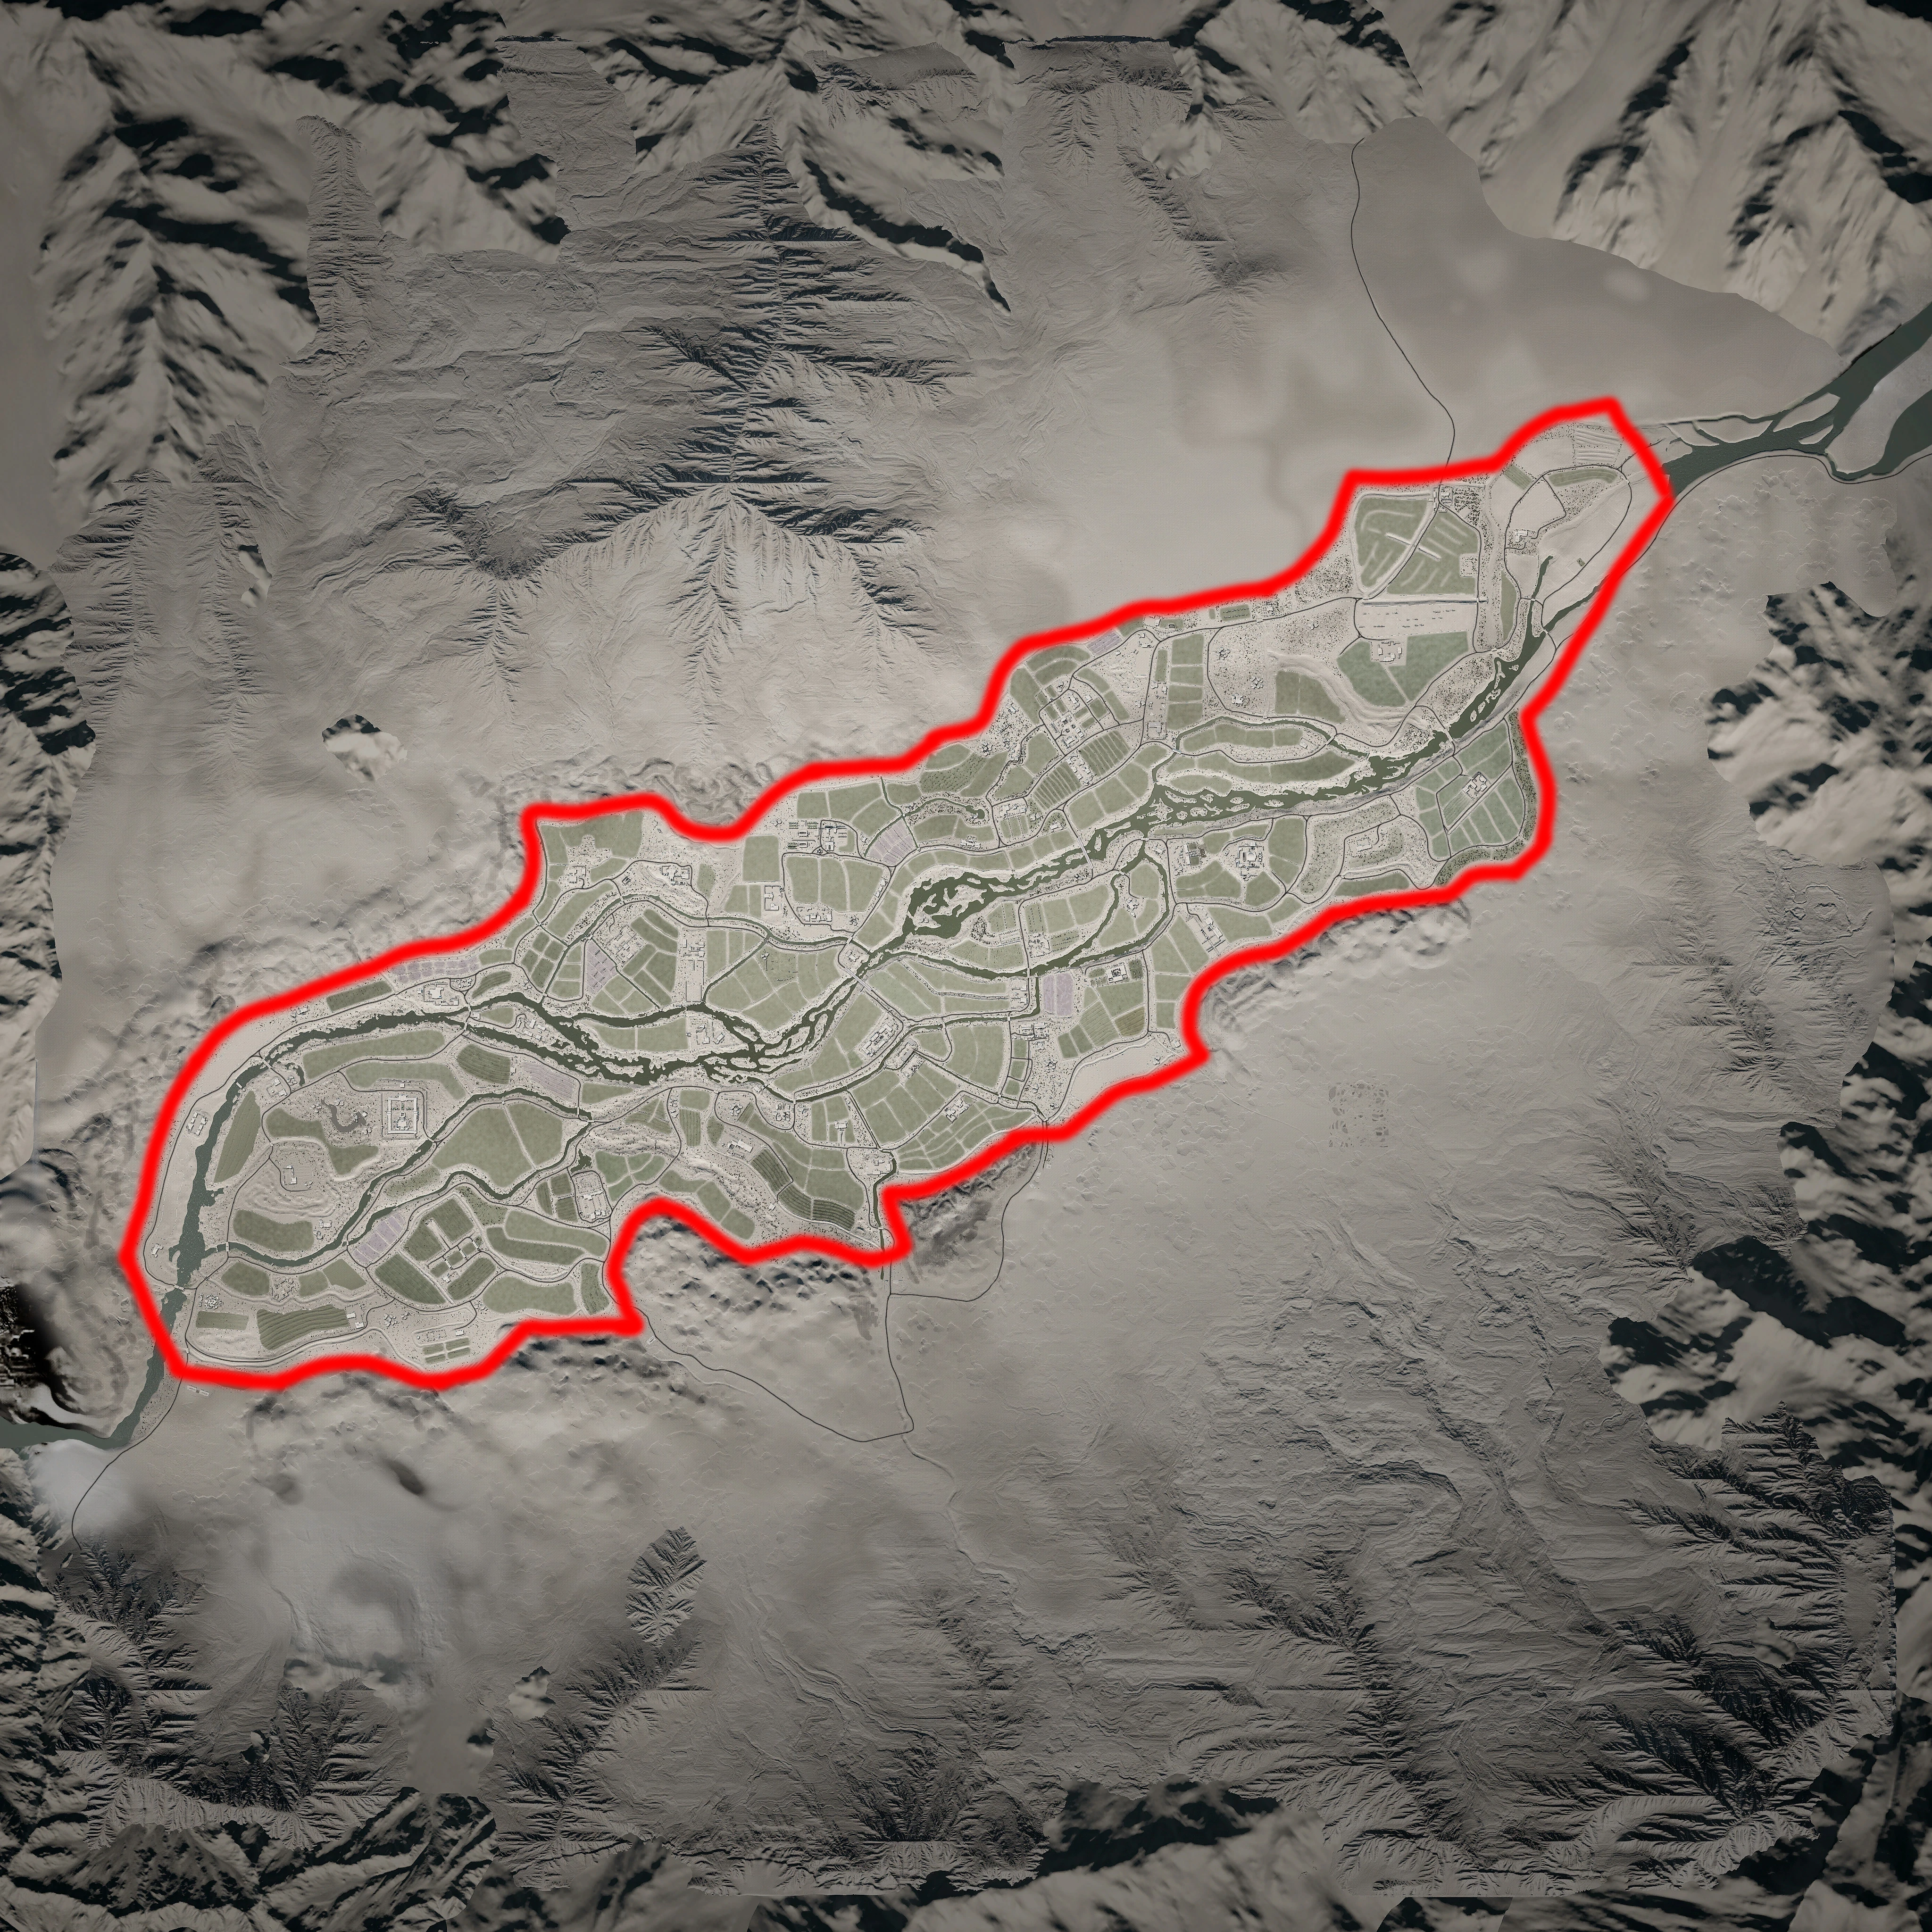
\includegraphics[width=0.8\textwidth]{chora_example.png}
    \caption{ChoraValley}
\end{figure}
Der tatsächliche Spielbereich, hier rot umrandet, nimmt nur einen Bruchteil der gesamten Map ein.\newline
Die offiziell angegebene Größe bezieht jedoch die gesamte Map mit ein, was Chora zu einer der größten Karten im Spiel machen würde.
Das ergibt im Sinne dieser Einteilung natürlich wenig Sinn.